%% USPSC-modelo-IFSCp.tex
% ---------------------------------------------------------------
% USPSC: Modelo de Trabalho Academico (tese de doutorado, dissertacao de
% mestrado e trabalhos monograficos em geral) em conformidade com 
% ABNT NBR 14724:2011: Informacao e documentacao - Trabalhos academicos -
% Apresentacao
%----------------------------------------------------------------
%% Esta \'e uma customiza\c{c}\~ao do abntex2-modelo-trabalho-academico.tex de v-1.9.5 laurocesar 
%% para as Unidades do Campus USP de S\~ao Carlos:
%% EESC - Escola de Engenharia de S\~ao Carlos
%% IAU - @[unidadefaculdade]@
%% ICMC - @[unidadefaculdade]@\^encias Matem\'aticas e de Computa\c{c}\~ao
%% IFSC - @[unidadefaculdade]@\'{\i}sica de S\~ao Carlos
%% IQSC - @[unidadefaculdade]@\'{\i}mica de S\~ao Carlos
%%
%% Este trabalho utiliza a classe USPSC.cls que \'e mantida pela seguinte equipe:
%% 
%% Coordena\c{c}\~ao e Programa\c{c}\~ao:
%%   - Marilza Aparecida Rodrigues Tognetti - marilza@sc.usp.br (PUSP-SC)
%%   - Ana Paula Aparecida Calabrez - aninha@sc.usp.br (PUSP-SC)
%% Normaliza\c{c}\~ao:
%%   - Brianda de Oliveira Ordonho Sigolo - brianda@usp.br (IAU)
%%   - Eduardo Graziosi Silva - edu.gs@sc.usp.br (EESC)
%%   - Eliana de C\'assia Aquareli Cordeiro - eliana@iqsc.usp.br (IQSC)
%%   - Fl\'avia Helena Cassin - cassinp@sc.usp.br (EESC)
%%   - Maria Cristina Cavarette Dziabas - mcdziaba@ifsc.usp.br (IFSC)
%%   - Regina C\'elia Vidal Medeiros - rcvmat@icmc.usp.br (ICMC)
%%
%% O USPSC-modelo.tex e USPSC-TCC-modelo.tex utilizam diversos arquivos relacionado em 
%% 2.1 Pacote USPSC: Classe USPSC e modelos de trabalhos acad\^emicos	do Tutorial do Pascote 
%%  USPSC para modelos de trabalhos de acad\^emicos em LaTeX - vers\~ao 3.1


%----------------------------------------------------------------
%% Sobre a classe abntex2.cls:
%% abntex2.cls, v-1.9.5 laurocesar
%% Copyright 2012-2015 by abnTeX2 group at https://www.abntex.net.br/ 
%%
%----------------------------------------------------------------

\documentclass[
% -- op\c{c}\~oes da classe memoir --
12pt,		% tamanho da fonte
openright,	% cap\'{\i}tulos come\c{c}am em p\'ag \'{\i}mpar (insere p\'agina vazia caso preciso)
twoside,  % para impress\~ao em anverso (frente) e verso. Oposto a oneside - Nota: utilizar \imprimirfolhaderosto*
%oneside, % para impress\~ao em p\'aginas separadas (somente anverso) -  Nota: utilizar \imprimirfolhaderosto
% inclua uma % antes do comando twoside e exclua a % antes do oneside 
a4paper,			% tamanho do papel. 
% -- op\c{c}\~oes da classe abntex2 --
chapter=TITLE,		% t\'{\i}tulos de cap\'{\i}tulos convertidos em letras mai\'usculas
% -- op\c{c}\~oes do pacote babel --
english,			% idioma adicional para hifeniza\c{c}\~ao
french,				% idioma adicional para hifeniza\c{c}\~ao
spanish,			% idioma adicional para hifeniza\c{c}\~ao
brazil				% o \'ultimo idioma \'e o principal do documento
% {USPSC-classe/USPSC} configura o cabe\c{c}alho contendo apenas o n\'umero da p\'agina
]{USPSC-classe/USPSC}
%]{USPSC-classe/USPSC1}
% Inclua % antes de ]{USPSC-classe/USPSC} e retire a % antes de %]{USPSC-classe/USPSC1} para utilizar o 
% cabe\c{c}alho diferenciado para as p\'aginas pares e \'{\i}mpares:
%- p\'aginas \'{\i}mpares: com se\c{c}\~oes ou subse\c{c}\~oes e o n\'umero da p\'agina
%- p\'aginas pares: com o n\'umero da p\'agina e o t\'{\i}tulo do cap\'{\i}tulo 
% ---
% ---
% Pacotes b\'asicos - Fundamentais 
% ---
\usepackage[T1]{fontenc}		% Sele\c{c}\~ao de c\'odigos de fonte.
\usepackage[utf8]{inputenc}		% Codifica\c{c}\~ao do documento (convers\~ao autom\'atica dos acentos)
\usepackage{lmodern}			% Usa a fonte Latin Modern
% Para utilizar a fonte Times New Roman, inclua uma % no in\'{\i}cio do comando acima  "\usepackage{lmodern}"
% Abaixo, tire a % antes do comando  \usepackage{times}
%\usepackage{times}		    	% Usa a fonte Times New Roman	
% Para usar a fonte , lembre-se de tirar a % do comando %\renewcommand{\ABNTEXchapterfont}{\rmfamily}, localizado mais abaixo, logo ap\'os "Outras op\c{c}\~oes para nota de rodap\'e no Sistema Num\'erico" 					
\usepackage{lastpage}			% Usado pela Ficha catalogr\'afica
\usepackage{indentfirst}		% Indenta o primeiro par\'agrafo de cada se\c{c}\~ao.
\usepackage{color}				% Controle das cores
\usepackage{graphicx}
\usepackage[export]{adjustbox}
\usepackage[skip=2pt,font=scriptsize]{caption}
\usepackage{subcaption}
\usepackage{soul}
			% Inclus\~ao de gr\'aficos
\usepackage{float} 				% Fixa tabelas e figuras no local exato
\usepackage{chemfig,chemmacros} % Para escrever rea\c{c}\~oes qu\'{\i}micas
\usepackage{tikz}				% Para escrever rea\c{c}\~oes qu\'{\i}micas e outros
\usetikzlibrary{positioning}
\usetikzlibrary{er}

\usepackage{microtype} 			% para melhorias de justifica\c{c}\~ao
\usepackage{pdfpages}
\usepackage{makeidx}            % para gerar \'{\i}ndice remissivo
\usepackage{hyphenat}          % Pacote para retirar a hifenizacao do texto
\usepackage[absolute]{textpos} % Pacote permite o posicionamento do texto
\usepackage{eso-pic}           % Pacote para incluir imagem de fundo
\usepackage{makebox}           % Pacote para criar caixa de texto
% ---

% ---
% Pacotes de cita\c{c}\~oes
% Cita\c{c}\~oes padr\~ao ABNT
% ---
% Sistemas de chamada: autor-data ou num\'erico.
% Sistema autor-data
%\usepackage[alf, abnt-emphasize=bf, abnt-thesis-year=both, abnt-repeated-author-omit=no, abnt-last-names=abnt, abnt-etal-cite, abnt-etal-list=3, abnt-etal-text=it, abnt-and-type=e, abnt-doi=doi, abnt-url-package=none, abnt-verbatim-entry=no]{abntex2cite}
%\bibliographystyle{USPSC-classe/abntex2-alf-USPSC}
% Se o idioma for o ingl\^es, exclua % no comando acima ou do comando abaixo
%\bibliographystyle{USPSC-classe/abntex2-alfeng-USPSC}

% Para o IQSC, que indica todos os autores nas refer\^encias, incluir % no in\'{\i}cio dos comandos acima e retirar a % dos comandos abaixo 
%\usepackage[alf, abnt-emphasize=bf, abnt-thesis-year=both, abnt-repeated-author-omit=no, abnt-last-names=abnt, abnt-etal-cite, abnt-etal-list=0, abnt-etal-text=it, abnt-and-type=e, abnt-doi=doi, abnt-url-package=none, abnt-verbatim-entry=no]{abntex2cite} 
%\bibliographystyle{USPSC-classe/abntex2-alf-USPSC}
% Se o idioma for o ingl\^es, exclua % no comando acima ou do comando abaixo
%\bibliographystyle{USPSC-classe/abntex2-alfeng-USPSC}

% Sistema Num\'erico
% Para cita\c{c}\~oes num\'ericas, sistema adotado pelo IFSC, incluir % no in\'{\i}cio dos comandos acima e retirar a % dos comandos abaixo 
\usepackage{cite}              % agrupa cita\c{c}\~oes num\'ericas consecutivas
\usepackage[num, abnt-emphasize=bf, abnt-thesis-year=both, abnt-repeated-author-omit=no, abnt-last-names=abnt, abnt-etal-cite, abnt-etal-list=3, abnt-etal-text=it, abnt-and-type=e, abnt-doi=doi, abnt-url-package=none, abnt-verbatim-entry=no]{abntex2cite} 
\bibliographystyle{USPSC-classe/abntex2-num-USPSC}
% Se o idioma for o ingl\^es, inclua % no comando acima e exclua o % do comando abaixo
%\bibliographystyle{USPSC-classe/abntex2-numeng-USPSC}

% Complementarmente, verifique as instru\c{c}\~oes abaixo sobre os Pacotes de Nota de rodap\'e
% ---
% Pacotes de Nota de rodap\'e
% Configura\c{c}\~oes de nota de rodap\'e

% O presente modelo adota o formato num\'erico para as notas de rodap\'es quando utiliza o sistema de chamada autor-data para cita\c{c}\~oes e refer\^encias. Para utilizar o sistema de chamada num\'erico para cita\c{c}\~oes e refer\^encias, habilitar um dos comandos abaixo.
% H\'a diversa op\c{c}\~oes para nota de rodap\'e no Sistema Num\'erico.  Para o IFSC, habilitade o comando abaixo.

\renewcommand{\thefootnote}{\fnsymbol{footnote}}  %Comando para inser\c{c}\~ao de s\'{\i}mbolos em nota de rodap\'e

% Outras op\c{c}\~oes para nota de rodap\'e no Sistema Num\'erico:
%\renewcommand{\thefootnote}{\alph{footnote}}      %Comando para inser\c{c}\~ao de letras min\'uscula em nota de rodap\'e
%\renewcommand{\thefootnote}{\Alph{footnote}}      %Comando para inser\c{c}\~ao de letras mai\'uscula em nota de rodap\'e
%\renewcommand{\thefootnote}{\roman{footnote}}     %Comando para inser\c{c}\~ao de n\'umeros romanos min\'usculos  em nota de rodap\'e
%\renewcommand{\thefootnote}{\Roman{footnote}}     %Comando para inser\c{c}\~ao de n\'umeros romanos min\'usculos  em nota de rodap\'e

\renewcommand{\footnotesize}{\small} %Comando para diminuir a fonte das notas de rodap\'e
%Para utilizar a fonte Times New Roman, inclua retire % do in\'{\i}cio do comando abaixo 
%\renewcommand{\ABNTEXchapterfont}{\rmfamily}

% ---
% Pacote para agrupar a cita\c{c}\~ao num\'erica consecutiva
% Quando for adotado o Sistema Num\'erico, a exemplo do IFSC, habilite 
% o pacote cite abaixo retirando a porcentagem antes do comando abaixo
%\usepackage[superscript]{cite}	

% ---
% Pacotes adicionais, usados apenas no \^ambito do Modelo Can\^onico do abnteX2
% ---
\usepackage{lipsum}				% para gera\c{c}\~ao de dummy text
% ---

% pacotes de tabelas
\usepackage{multicol}	% Suporte a mesclagens em colunas
\usepackage{multirow}	% Suporte a mesclagens em linhas
\usepackage{longtable}	% Tabelas com v\'arias p\'aginas
\usepackage{threeparttablex}    % notas no longtable
\usepackage{array}

% ----
% Compatibiliza\c{c}\~ao com a ABNT NBR 6023:2018
% Para tirar <> da URL
%\DeclareFieldFormat{url}{\bibstring{urlfrom}\addcolon\addspace\url{#1}}
\usepackage{USPSC-classe/ABNT6023-2018}
% As demais compatibiliza\c{c}\~oes est\~ao nos arquivos abntex2-alf-USPSC.bst e abntex2-num-USPSC.bst, chamados atrav\'es do comando \bibliographystyle{USPSC-classe/abntex2-alf-USPSC} ou %\bibliographystyle{USPSC-classe/abntex2-num-USPSC}, dependendo se o Sistemas de chamada for autor-data ou num\'erico.
% ----


% ---
% DADOS INICIAIS - Define sigla com t\'{\i}tulo, \'area de concentra\c{c}\~ao e op\c{c}\~ao do Programa 
% Consulte a tabela referente aos Programas, \'areas e op\c{c}\~oes de sua unidade contante do
% arquivo USPSC-Siglas estabelecidas para os Programas de P\'os-Gradua\c{c}\~ao nos AP\^ENDICES B-J
\siglaunidade{IFSC}
\programa{DFAp}
% Os demais dados dever\~ao ser fornecidos no arquivo USPSC-pre-textual-UUUU ou USPSC-TCC-pre-textual-UUUU, onde UUUU \'e a sigla da Unidade. 
% Exemplo:USPSC-pre-textual-IFSC.tex
% ---
% Configura\c{c}\~oes de apar\^encia do PDF final
% alterando o aspecto da cor azul
\definecolor{blue}{RGB}{41,5,195}

% informa\c{c}\~oes do PDF
\makeatletter
\hypersetup{
	%pagebackref=true,
	pdftitle={\@title}, 
	pdfauthor={\@author},
	pdfsubject={\imprimirpreambulo},
	pdfcreator={LaTeX with abnTeX2},
	pdfkeywords={abnt}{latex}{abntex}{USPSC}{trabalho acad\^emico}, 
	colorlinks=true,       		% false: boxed links; true: colored links
	linkcolor=black,          	% color of internal links
	citecolor=black,        		% color of links to bibliography
	filecolor=black,      		% color of file links
	urlcolor=black,
	%Para habilitar as cores dos links, retire a % antes dos comandos abaixo e inclua a % antes das 4 linhas de comando acima 
	%linkcolor=blue,            	% color of internal links
	%citecolor=blue,        		% color of links to bibliography
	%filecolor=magenta,      		% color of file links
	%urlcolor=blue,
	bookmarksdepth=4	
}
\makeatother
% --- 
% --- 
% Espa\c{c}amentos entre linhas e par\'agrafos 
% --- 

% O tamanho do par\'agrafo \'e dado por:
\setlength{\parindent}{1.3cm}

% Controle do espa\c{c}amento entre um par\'agrafo e outro:
\setlength{\parskip}{0.2cm}  % tente tamb\'em \onelineskip

% ---
% compila o sum\'ario e \'{\i}ndice
\makeindex
% ---

% ----
% In\'{\i}cio do documento
% ----
\begin{document}

% Seleciona o idioma do documento (conforme pacotes do babel)
\selectlanguage{brazil}
% Se o idioma do texto for ingl\^es, inclua uma % antes do 
%      comando \selectlanguage{brazil} e 
%      retire a % antes do comando abaixo
%\selectlanguage{english}

% Retira espa\c{c}o extra obsoleto entre as frases.
\frenchspacing 

% --- Formata\c{c}\~ao dos T\'{\i}tulos
\renewcommand{\ABNTEXchapterfontsize}{\fontsize{12}{12}\bfseries}
\renewcommand{\ABNTEXsectionfontsize}{\fontsize{12}{12}\bfseries}
\renewcommand{\ABNTEXsubsectionfontsize}{\fontsize{12}{12}\normalfont}
\renewcommand{\ABNTEXsubsubsectionfontsize}{\fontsize{12}{12}\normalfont}
\renewcommand{\ABNTEXsubsubsubsectionfontsize}{\fontsize{12}{12}\normalfont}


% ----------------------------------------------------------
% ELEMENTOS PR\'E-TEXTUAIS
% ----------------------------------------------------------
% ---
% Capa
% ---
\imprimircapa
% ---
% Folha de rosto
% (o * indica impress\~ao em anverso (frente) e verso )
% ---
\imprimirfolhaderosto*
%\imprimirfolhaderosto
% ---
% ---
% Inserir a ficha catalogr\'afica em pdf
% ---
% A biblioteca da sua Unidade lhe fornecer\'a um PDF com a ficha
% catalogr\'afica definitiva. 
% Quando estiver com o documento, salve-o como PDF no diret\'orio
% do seu projeto como fichacatalografica.pdf e inclua o arquivo
% utilizando o comando abaixo:

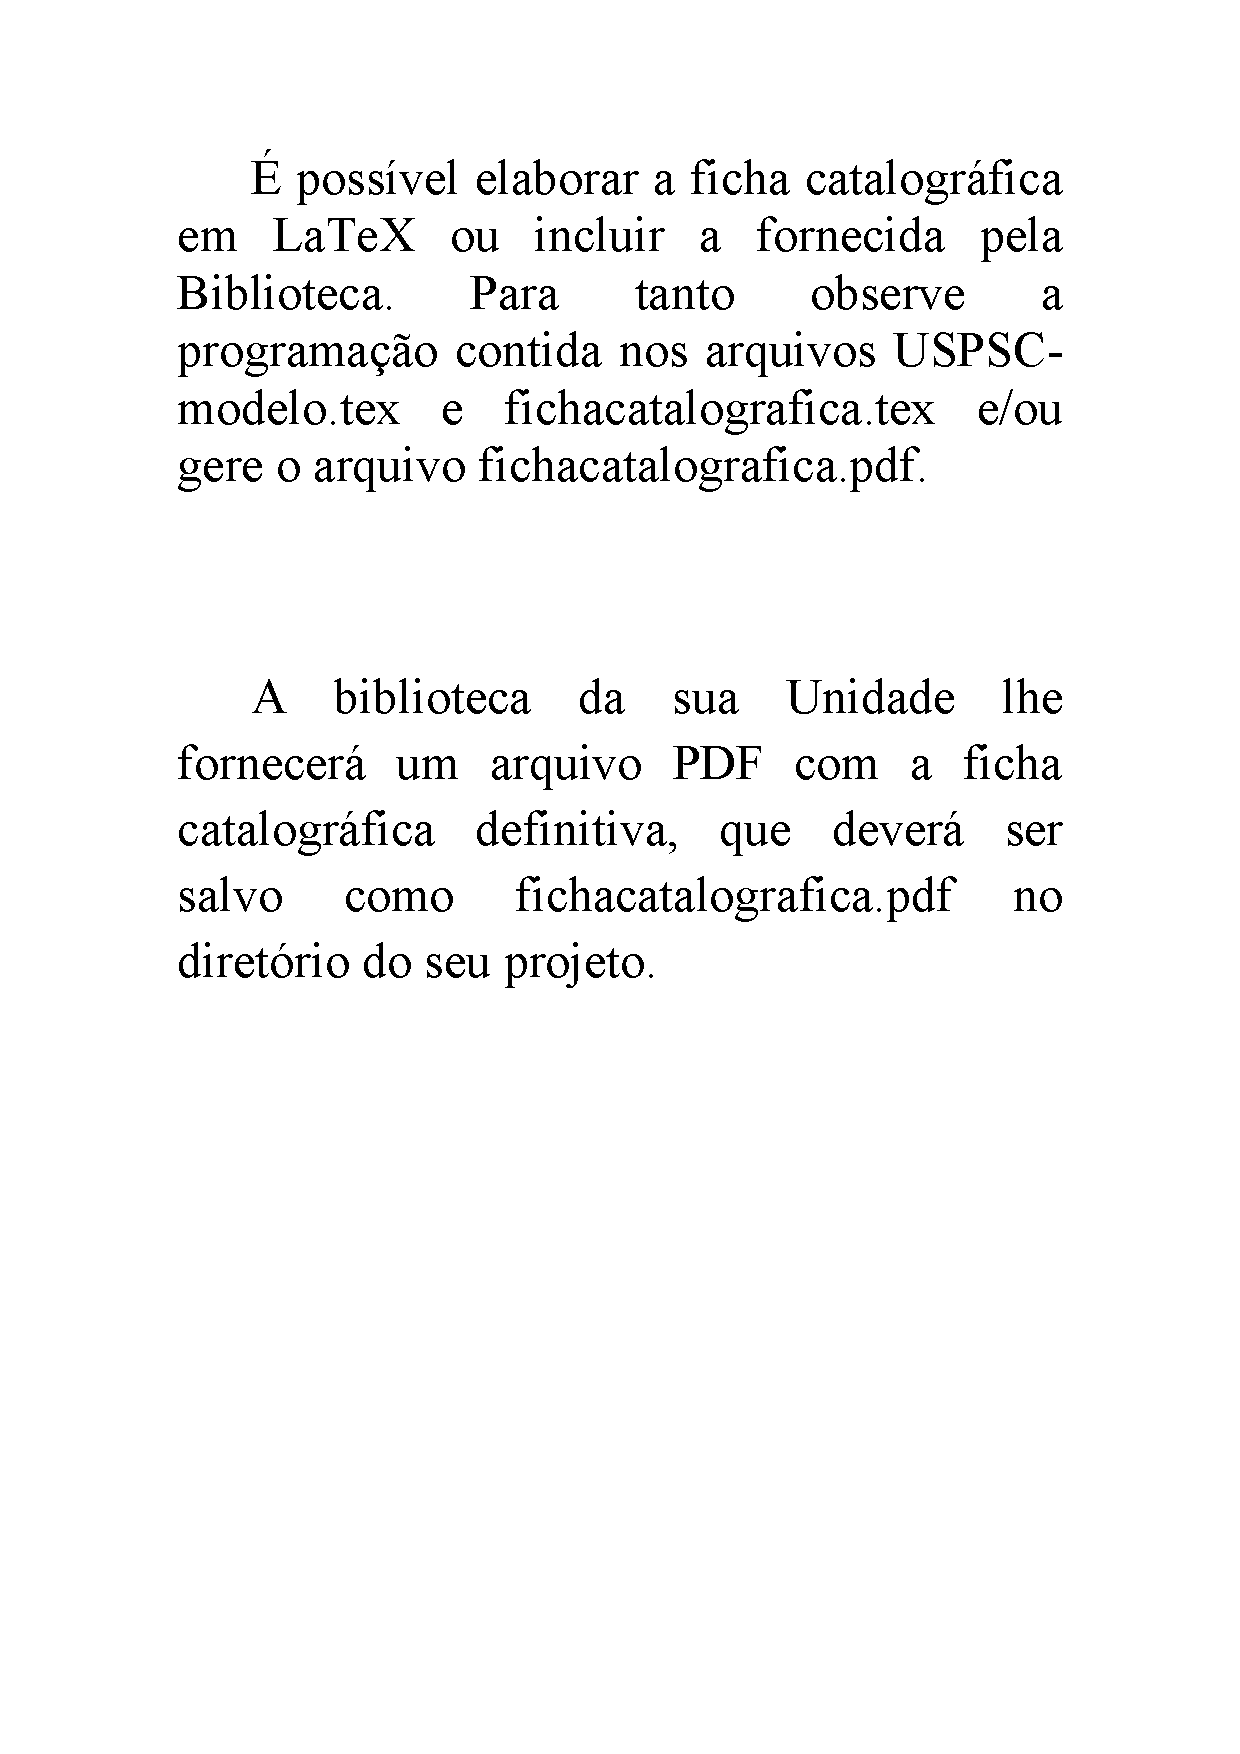
\includepdf{USPSC-TA-PreTextual/USPSC-fichacatalografica.pdf}

% Se voc\^e optar por elaborar a ficha catalogr\'afica, dever\'a 
% incluir uma % antes da linha % antes
% do comando %% USPSC-fichacatalografica.tex
% ---
% Inserir a ficha bibliografica
% ---
% Isto \'e um exemplo de Ficha Catalogr\'afica, ou ``Dados internacionais de
% cataloga\c{c}\~ao-na-publica\c{c}\~ao''. Voc\^e pode utilizar este modelo como refer\^encia. 
% Por\'em, provavelmente a biblioteca da sua universidade lhe fornecer\'a um PDF
% com a ficha catalogr\'afica definitiva ap\'os a defesa do trabalho. Quando estiver
% com o documento, salve-o como PDF no diret\'orio do seu projeto e substitua todo
% o conte\'udo de implementa\c{c}\~ao deste arquivo pelo comando abaixo:
%
\begin{fichacatalografica}
	\hspace{-1.4cm}
	\imprimirnotaautorizacao \\ \\
	%\sffamily
	\vspace*{\fill}					% Posi\c{c}\~ao vertical
\begin{center}					% Minipage Centralizado
  \imprimirnotabib \\
  \begin{table}[htb]
	\scriptsize
	\centering	
	\begin{tabular}{|p{0.9cm} p{8.7cm}|}
		\hline
	      & \\
		  &	  \imprimirautorficha     \\
		
		 \imprimircutter & 
							\hspace{0.4cm}\imprimirtitulo~  / ~\imprimirautor~ ;  ~\imprimirorientadorcorpoficha. -- 	\imprimirlocal, \imprimirdata.   \\
		
		  &  % Para incluir nota referente \`a vers\~ao corrigida no corpo da ficha,
			  % incluir % no in\'{\i}cio da linha acima e tirar a % do in\'{\i}cio da linha abaixo
			  %	\hspace{0.4cm} \imprimirtitulo~  / ~\imprimirautor~ ; ~\imprimirorientadorcorpoficha~- ~\imprimirnotafolharosto. -- \imprimirlocal, \imprimirdata.  \\
		
			\hspace{0.4cm}\pageref{LastPage} p. : il. (algumas color.) ; 30 cm.\\ 
		  & \\
		  & 
		    \hspace{0.4cm}\imprimirnotaficha ~--~ 
						  \imprimirunidademin, 
						  \imprimiruniversidademin, 
		                  \imprimirdata. \\ 
		  & \\                 
		   % Para incluir nota referente \`a vers\~ao corrigida em notas,
		    % incluir uma % no in\'{\i}cio da linha acima e	
		    % tirar a % do in\'{\i}cio da linha abaixo
		    % & \hspace{0.4cm}\imprimirnotafolharosto \\ 
		  & \\ 
		  & \hspace{0.4cm}1. LaTeX. 2. abnTeX. 3. Classe USPSC. 4. Editora\c{c}\~ao de texto. 5. Normaliza\c{c}\~ao da documenta\c{c}\~ao. 6. Tese. 7. Disserta\c{c}\~ao. 8. Documentos (elabora\c{c}\~ao). 9. Documentos eletr\^onicos. I. \imprimirorientadorficha. 
		   II. T\'{\i}tulo. \\
	
		     %Se houver co-orientador, inclua % antes da linha (antes de II. T\'{\i}tulo.) 
		     %          e tire a % antes do comando abaixo 
		     %III. T\'{\i}tulo. \\   
		  \hline
	\end{tabular}
  \end{table}
\end{center}
\end{fichacatalografica}
% ---

 
% e retirar o % do comando abaixo
%%% USPSC-fichacatalografica.tex
% ---
% Inserir a ficha bibliografica
% ---
% Isto \'e um exemplo de Ficha Catalogr\'afica, ou ``Dados internacionais de
% cataloga\c{c}\~ao-na-publica\c{c}\~ao''. Voc\^e pode utilizar este modelo como refer\^encia. 
% Por\'em, provavelmente a biblioteca da sua universidade lhe fornecer\'a um PDF
% com a ficha catalogr\'afica definitiva ap\'os a defesa do trabalho. Quando estiver
% com o documento, salve-o como PDF no diret\'orio do seu projeto e substitua todo
% o conte\'udo de implementa\c{c}\~ao deste arquivo pelo comando abaixo:
%
\begin{fichacatalografica}
	\hspace{-1.4cm}
	\imprimirnotaautorizacao \\ \\
	%\sffamily
	\vspace*{\fill}					% Posi\c{c}\~ao vertical
\begin{center}					% Minipage Centralizado
  \imprimirnotabib \\
  \begin{table}[htb]
	\scriptsize
	\centering	
	\begin{tabular}{|p{0.9cm} p{8.7cm}|}
		\hline
	      & \\
		  &	  \imprimirautorficha     \\
		
		 \imprimircutter & 
							\hspace{0.4cm}\imprimirtitulo~  / ~\imprimirautor~ ;  ~\imprimirorientadorcorpoficha. -- 	\imprimirlocal, \imprimirdata.   \\
		
		  &  % Para incluir nota referente \`a vers\~ao corrigida no corpo da ficha,
			  % incluir % no in\'{\i}cio da linha acima e tirar a % do in\'{\i}cio da linha abaixo
			  %	\hspace{0.4cm} \imprimirtitulo~  / ~\imprimirautor~ ; ~\imprimirorientadorcorpoficha~- ~\imprimirnotafolharosto. -- \imprimirlocal, \imprimirdata.  \\
		
			\hspace{0.4cm}\pageref{LastPage} p. : il. (algumas color.) ; 30 cm.\\ 
		  & \\
		  & 
		    \hspace{0.4cm}\imprimirnotaficha ~--~ 
						  \imprimirunidademin, 
						  \imprimiruniversidademin, 
		                  \imprimirdata. \\ 
		  & \\                 
		   % Para incluir nota referente \`a vers\~ao corrigida em notas,
		    % incluir uma % no in\'{\i}cio da linha acima e	
		    % tirar a % do in\'{\i}cio da linha abaixo
		    % & \hspace{0.4cm}\imprimirnotafolharosto \\ 
		  & \\ 
		  & \hspace{0.4cm}1. LaTeX. 2. abnTeX. 3. Classe USPSC. 4. Editora\c{c}\~ao de texto. 5. Normaliza\c{c}\~ao da documenta\c{c}\~ao. 6. Tese. 7. Disserta\c{c}\~ao. 8. Documentos (elabora\c{c}\~ao). 9. Documentos eletr\^onicos. I. \imprimirorientadorficha. 
		   II. T\'{\i}tulo. \\
	
		     %Se houver co-orientador, inclua % antes da linha (antes de II. T\'{\i}tulo.) 
		     %          e tire a % antes do comando abaixo 
		     %III. T\'{\i}tulo. \\   
		  \hline
	\end{tabular}
  \end{table}
\end{center}
\end{fichacatalografica}
% ---


% As informa\c{c}\~oes que comp\~oem a ficha catalogr\'afica est\~ao 
% definidas no arquivo USPSC-pre-textual-UUUU.tex
% ---

% ---
% Folha de rosto adicional
% Para imprimir a folha de rosto adicional, exigida por algumas Unidades, a exemplo do ICMC,
% retire a % antes do comando abaixo

%\imprimirfolhaderostoadic

% ---
% ---
% Inserir errata
% ---

%% USPSC-Errata.tex
\begin{errata}
	%\OnehalfSpacing 			
	A errata é um elemento opcional, que consiste de uma lista de erros da obra, precedidos pelas folhas e linhas onde eles ocorrem e seguidos pelas correções correspondentes. Deve ser inserida logo após a folha de rosto e conter a referência do trabalho para facilitar sua identificação, conforme a ABNT NBR 14724 \cite{nbr14724}.
	
	Modelo de Errata:
		
	\begin{flushleft} 
			\setlength{\absparsep}{0pt} % ajusta o espaçamento da referência	
			\SingleSpacing 
			\imprimirautorabr~ ~\textbf{\imprimirtituloresumo}.	\imprimirdata. \pageref{LastPage}p. 
			%Substitua p. por f. quando utilizar oneside em \documentclass
			%\pageref{LastPage}f.
			\imprimirtipotrabalho~-~\imprimirinstituicao, \imprimirlocal, \imprimirdata. 
 	\end{flushleft}
\vspace{\onelineskip}
\OnehalfSpacing 
\center
\textbf{ERRATA}
\vspace{\onelineskip}
\OnehalfSpacing 
\begin{table}[htb]
	\center
	\footnotesize
	\begin{tabular}{p{2cm} p{2cm} p{4cm} p{4cm} }
		\hline
		\textbf{Folha} & \textbf{Linha}  & \textbf{Onde se lê}  & \textbf{Leia-se}  \\
			\hline
			1 & 10 & auto-conclavo & autoconclavo\\
		\hline
	\end{tabular}
\end{table}
\end{errata}
% ---

% ---

% ---
% Inserir folha de aprova\c{c}\~ao
% ---

% A Folha de aprova\c{c}\~ao \'e um elemento obrigat\'orio da NBR 4724/2011 (se\c{c}\~ao 4.2.1.3). 
% Ap\'os a defesa/aprova\c{c}\~ao do trabalho, gere o arquivo folhadeaprovacao.pdf da p\'agina assinada pela banca 
% e iclua o arquivo utilizando o comando abaixo:
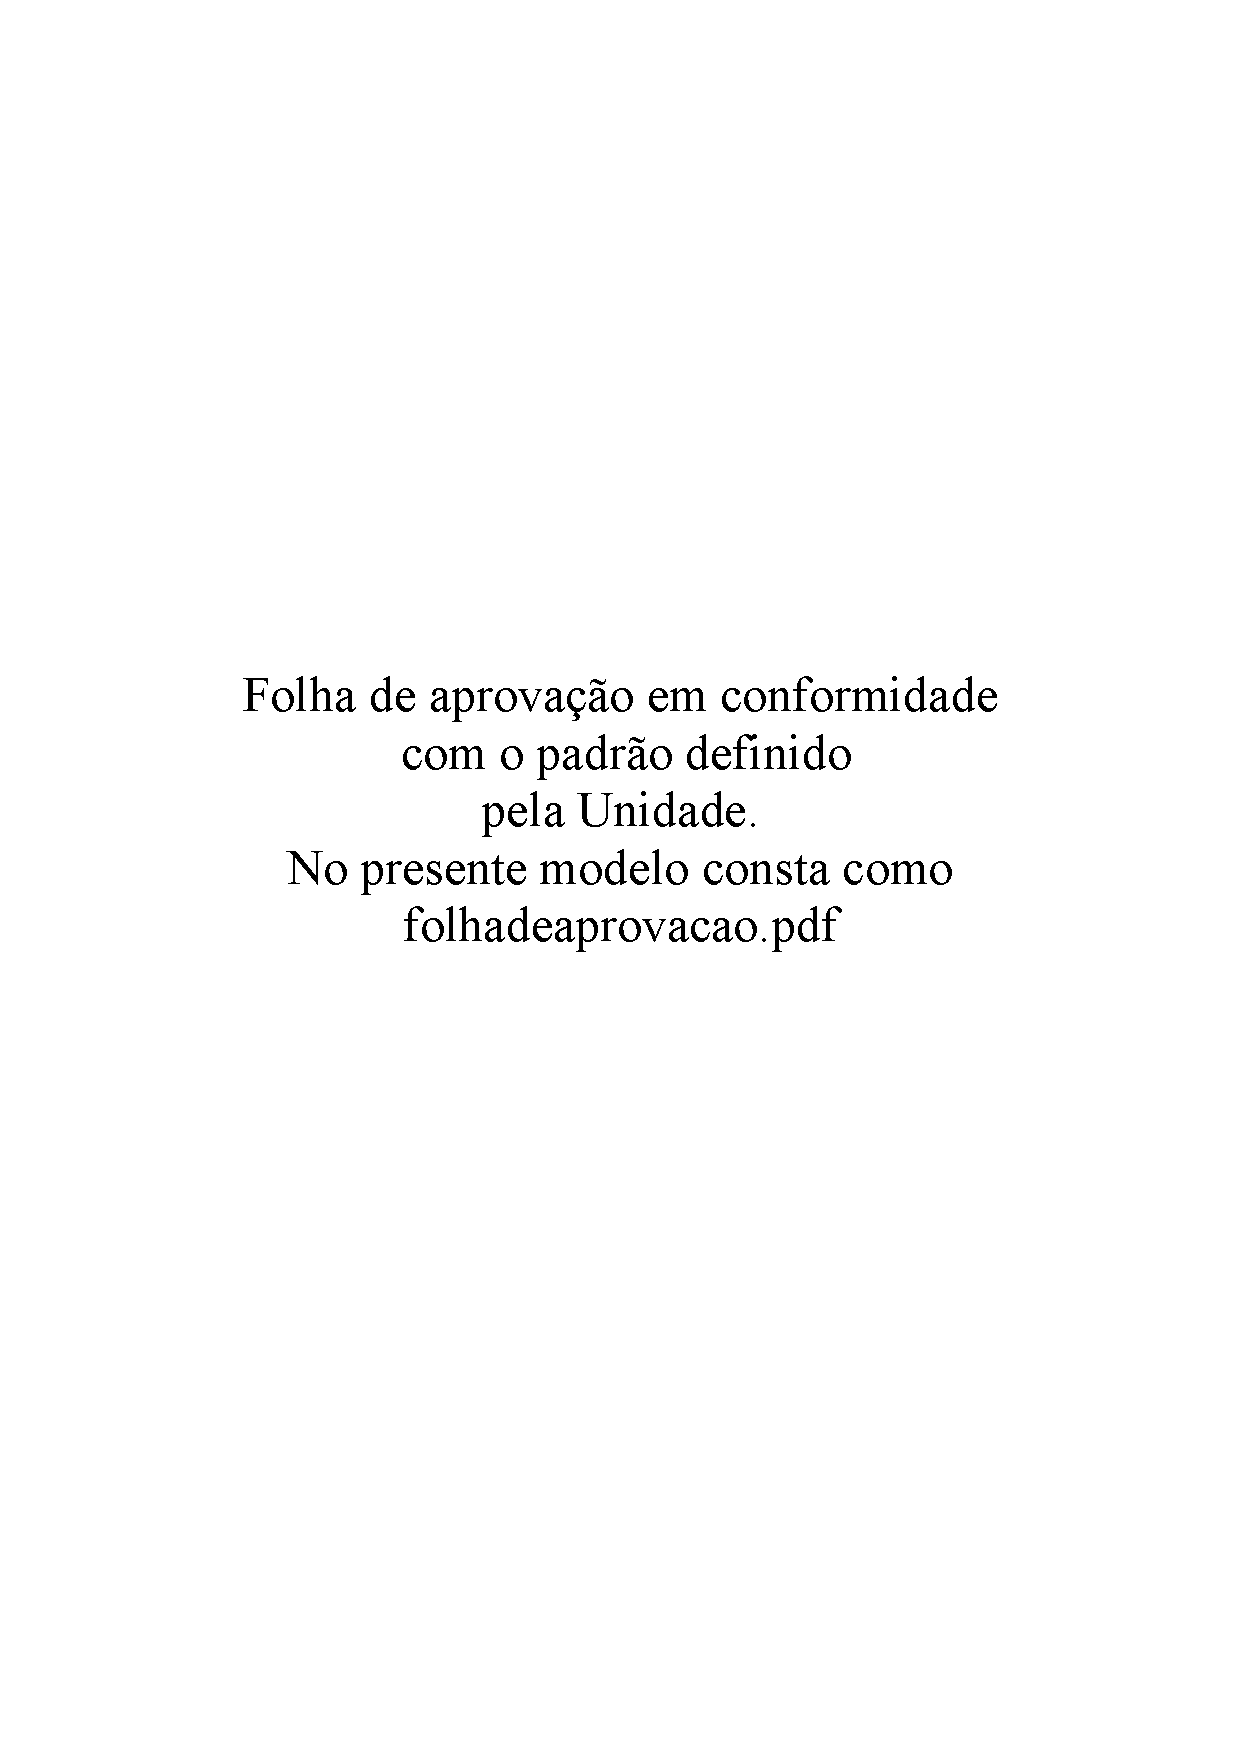
\includepdf{USPSC-TA-PreTextual/USPSC-folhadeaprovacao.pdf}
% Alternativa para a Folha de Aprova\c{c}\~ao:
% Se for a sua op\c{c}\~ao elaborar uma folha de aprova\c{c}\~ao, insira uma % antes do comando acima que inclui o arquivo folhadeaprovacao.pdf,
% tire o % do comando abaixo e altere o arquivo folhadeaprovacao.tex conforme suas necessidades
%\include{folhadeaprovacao}

\includepdf{USPSC-TA-PreTextual/USPSC-PaginaEmBranco.pdf}

% ---
% Dedicat\'oria
% ---
%% USPSC-Dedicatoria.tex
\begin{dedicatoria}
   \vspace*{\fill}
   \centering
   \noindent\textit{@[dedicatoria]@} \vspace*{\fill}
\end{dedicatoria}
% ---
% ---

% ---
% Agradecimentos
% ---
%% USPSC-Agradecimentos.tex
\begin{agradecimentos}
	Primeira frase do agradecimento ....
	
	Segunda frase ....
	
	Outras frases ....
	
	Última frase ....
	
\end{agradecimentos}
% ---
% ---

% ---
% Ep\'{\i}grafe
% ---
%% USPSC-Epigrafe.tex
\begin{epigrafe}
    \vspace*{\fill}
	\begin{flushright}
		\textit{``O estudo, a busca da verdade e da beleza são domínios \\
		em que nos \'e consentido sermos crianças por toda a vida.''\\
		Albert Einstein}
	\end{flushright}
\end{epigrafe}
% ---
% ---

% A T E N \c{C} \~A O
% Se o idioma do texto for em ingl\^es, o abstract deve preceder o resumo
% resumo em portugu\^es
%
% Resumo
% ---
%% USPSC-Resumo.tex
\setlength{\absparsep}{18pt} % ajusta o espaçamento dos parágrafos do resumo		
\begin{resumo}
	\begin{flushleft} 
			\setlength{\absparsep}{0pt} % ajusta o espaçamento da referência	
			\SingleSpacing 
			\imprimirautorabr~~\textbf{\imprimirtituloresumo}.	\imprimirdata. \pageref{LastPage}p. 
			%Substitua p. por f. quando utilizar oneside em \documentclass
			%\pageref{LastPage}f.
			\imprimirtipotrabalho~-~\imprimirinstituicao, \imprimirlocal, \imprimirdata. 
 	\end{flushleft}
\OnehalfSpacing 			
 O resumo deve ressaltar o  objetivo, o método, os resultados e as conclusões do documento. A ordem e a extensão  destes itens dependem do tipo de resumo (informativo ou indicativo) e do  tratamento que cada item recebe no documento original. O resumo deve ser
 precedido da referência do documento, com exceção do resumo inserido no
 próprio documento. (\ldots)  Salientamos que algumas Unidades exigem o titulo dos trabalhos acadêmicos em inglês, tornando necessário a inclusão das referências nos resumos e abstracts, o que foi adotado no \textbf{Modelo para TCC em \LaTeX\ utilizando a classe USPSC} e no \textbf{Modelo para teses e dissertações em \LaTeX\ utilizando a classe USPSC}. As palavras-chave devem figurar logo abaixo do  resumo, antecedidas da expressão Palavras-chave:, separadas entre si por  ponto e finalizadas também por ponto \cite{nbr6028}.
 

 \textbf{Palavras-chave}: LaTeX. Classe USPSC. Tese. Dissertação. Trabalho de conclusão de curso (TCC). 
\end{resumo}
% ---

% Abstract
% ---
%% USPSC-Abstract.tex
%\autor{Silva, M. J.}
\begin{resumo}[Abstract]
 \begin{otherlanguage*}{english}
	\begin{flushleft} 
		\setlength{\absparsep}{0pt} % ajusta o espa\c{c}amento dos par\'agrafos do resumo		
 		\SingleSpacing  		\imprimirautorabr~~\textbf{\imprimirtitleabstract}.	\imprimirdata.  \pageref{LastPage}p. 
		%Substitua p. por f. quando utilizar oneside em \documentclass
		%\pageref{LastPage}f.
		\imprimirtipotrabalhoabs~-~\imprimirinstituicao, \imprimirlocal, 	\imprimirdata. 
 	\end{flushleft}
	\OnehalfSpacing 
   This is the english abstract.

   \vspace{\onelineskip}
 
   \noindent 
   \textbf{Keywords}: LaTeX. USPSC class. Thesis. Dissertation. Conclusion course paper. 
 \end{otherlanguage*}
\end{resumo}

% ---

% ---
% inserir lista de figurass
% ---
\pdfbookmark[0]{\listfigurename}{lof}
\listoffigures*
\cleardoublepage
% ---

% ---
% inserir lista de tabelas
% ---
\pdfbookmark[0]{\listtablename}{lot}
\listoftables*
\cleardoublepage
% ---

% ---
% inserir lista de quadros
% ---
\pdfbookmark[0]{\listofquadroname}{loq}
\listofquadro*
\cleardoublepage
% ---

% ---
% inserir lista de abreviaturas e siglas
% ---
% USPSC-AbreviaturasSiglas.tex
\begin{siglas}
    \item[ABNT] Associação Brasileira de Normas Técnicas
    \item[abnTeX] ABsurdas Normas para TeX
	\item[IBGE] Instituto Brasileiro de Geografia e Estatística
	\item[LaTeX] Lamport TeX
	\item[USP] Universidade de São Paulo
	\item[USPSC] Campus USP de São Carlos
\end{siglas}

% ---

% ---
% inserir lista de s\'{\i}mbolos
% ---
% USPSC-Simbolos.tex
\begin{simbolos}
  \item[$ \Gamma $] Letra grega Gama
  \item[$ \Lambda $] Lambda
  \item[$ \zeta $] Letra grega minúscula zeta
  \item[$ \in $] Pertence
\end{simbolos}
% ---
% ---
% inserir o sumario
% ---
\pdfbookmark[0]{\contentsname}{toc}
\tableofcontents*
\cleardoublepage
% ---
% ----------------------------------------------------------
% ELEMENTOS TEXTUAIS
% ----------------------------------------------------------
\textual
% Os cap\'{\i}tulos s\~ao inseridos como arquivos externos 

% Cap\'{\i}tulo 1 - Introdu\c{c}\~ao
% ---
%% USPSC-Introducao.tex

% ----------------------------------------------------------
% Introdução (exemplo de capítulo sem numeração, mas presente no Sum\'ario)
% ----------------------------------------------------------
\chapter[Introdução]{Introdução}
\label{Introdução}


Parte inicial do texto, que cont\'em a delimitação do assunto tratado, objetivos da pesquisa e outros elementos necess\'arios para apresentar o tema do trabalho \cite{aguia2020}.



h\'{\i}pica
H\'IPICA
ch\~ao
CH\~AO
\'OPTICA
\'optica
PARLAPAT\~OES

\'a
\'A
\`a
\`A
\~a
\~A
\^a
\^A
\'e
\'E
\^e
\^E
\'{\i}
\'I
\'o
\'O
\~o
\~O
\^o
\^O
\'u
\'U
\c{c}
\c{C}

parlapat\~oes


pa\c{c}oca
fa\c{c}a




	

% ---

% ---
% Cap\'{\i}tulo 2
% ---
%% USPSC-Cap2-Desenvolvimento.tex 

% ---
% Este capítulo, utilizado por diferentes exemplos do abnTeX2, ilustra o uso de
% comandos do abnTeX2 e de LaTeX.
% ---

\chapter{Desenvolvimento}\label{cap_exemplos}
Este capítulo é parte principal do trabalho acadêmico e deve conter a exposição ordenada e detalhada do assunto. Divide-se em seções e subseções, em conformidade com a abordagem do tema e do método, abrangendo: revisão bibliográfica, materiais e métodos, técnicas utilizadas, resultados obtidos e discussão.

Abaixo são apresentados minimamente exemplos tabelas, quadros, divisões de documentos e outros itens. Consulte o \textbf{Tutorial do Pacote USPSC para modelos de trabalhos de acad\^emicos em LaTeX - vers\~ao 3.1} para demais informações. 

\section{Resultados de comandos}\label{sec-divisoes}

% ---
\subsection{Tabelas e quadros}

O \textbf{Tutorial do Pacote USPSC para modelos de trabalhos de acad\^emicos em LaTeX - vers\~ao 3.1} apresenta orientações completas e diversas formatações de tabelas, dentre elas a \autoref{tab-ibge}, que é um exemplo de tabela alinhada que pode ser longa ou curta, conforme padrão do Instituto Brasileiro de Geografia e Estatística (IBGE).

%\begin{table}[H]
\begin{table}[htb]
	\IBGEtab{%
		\caption{Frequência anual por categoria de usuários}%
		\label{tab-ibge}
	}{%
		\begin{tabular}{ccc}
			\toprule
			Categoria de Usuários & Frequência de Usuários \\
			\midrule \midrule
			Graduação & 72\% \\
			\midrule 
			Pós-Graduação & 15\% \\
			\midrule 
			Docente & 10\% \\
			\midrule 
			Outras & 3\% \\
			\bottomrule
		\end{tabular}%
	}{%
		\fonte{Elaborada pelos autores.}%
		\nota{Exemplo de uma nota.}%
		\nota[Anotações]{Uma anotação adicional, que pode ser seguida de várias
			outras.}%
		
	}
\end{table}


A formatação do quadro é similar à tabela, mas deve ter suas laterais fechadas e conter as linhas horizontais.
\newpage

% o comando \newpage foi utilizado para forçar a quebra de página

\begin{quadro}[htb]
	\caption{\label{quadro_modelo}Níveis de investigação}
	\begin{tabular}{|p{2.6cm}|p{6.0cm}|p{2.25cm}|p{3.40cm}|}
		\hline
		\textbf{Nível de Investigação} & \textbf{Insumos}  & \textbf{Sistemas de Investigação}  & \textbf{Produtos}  \\
		\hline
		Meta-nível & Filosofia\index{filosofia} da Ciência  & Epistemologia &
		Paradigma  \\
		\hline
		Nível do objeto & Paradigmas do metanível e evidências do nível inferior &
		Ciência  & Teorias e modelos \\
		\hline
		Nível inferior & Modelos e métodos do nível do objeto e problemas do nível inferior & Prática & Solução de problemas  \\
		\hline
	\end{tabular}
	\begin{flushleft}
		%\fonte{\citeonline{van1986}}
		Fonte: \citeonline{van1986}
	\end{flushleft}
\end{quadro} 


No \textbf{Tutorial do Pacote USPSC para modelos de trabalhos de acad\^emicos em LaTeX - vers\~ao 3.1} são apresentados mais exemplos de quadros.

% ---
\subsection{Figuras}\label{sec_figuras}
% ---
\index{figuras}Figuras podem ser criadas diretamente em \LaTeX,
como o exemplo da \autoref{fig_circulo}. \\ 

\begin{figure}[htb]
	\caption{\label{fig_circulo}A delimitação do espaço}
	\begin{center}
		\setlength{\unitlength}{9cm}
		\begin{picture}(1,1)
		\put(0,0){\line(0,1){1}}
		\put(0,0){\line(1,0){1}}
		\put(0,0){\line(1,1){1}}
		\put(0,0){\line(1,2){.5}}
		\put(0,0){\line(1,3){.3333}}
		\put(0,0){\line(1,4){.25}}
		\put(0,0){\line(1,5){.2}}
		\put(0,0){\line(1,6){.1667}}
		\put(0,0){\line(2,1){1}}
		\put(0,0){\line(2,3){.6667}}
		\put(0,0){\line(2,5){.4}}
		\put(0,0){\line(3,1){1}}
		\put(0,0){\line(3,2){1}}
		\put(0,0){\line(3,4){.75}}
		\put(0,0){\line(3,5){.6}}
		\put(0,0){\line(4,1){1}}
		\put(0,0){\line(4,3){1}}
		\put(0,0){\line(4,5){.8}}
		\put(0,0){\line(5,1){1}}
		\put(0,0){\line(5,2){1}}
		\put(0,0){\line(5,3){1}}
		\put(0,0){\line(5,4){1}}
		\put(0,0){\line(5,6){.8333}}
		\put(0,0){\line(6,1){1}}
		\put(0,0){\line(6,5){1}}
		\end{picture}
	\end{center}
	\legend{Fonte: \citeonline{equipeabntex2}}
\end{figure}

Consulte o \textbf{Tutorial do Pacote USPSC para modelos de trabalhos de acad\^emicos em LaTeX - vers\~ao 3.1} para conhecer mais recursos referentes à figuras. 

% ---
\section{Divisões do documento}\label{sec-divisoes-b}
Esta seção exemplifica o uso de divisões de documentos em conformidade com a ABNT NBR 6024  \cite{nbr6024}.
% ---
% ---
\subsection{Divisões do documento: subseção}\label{sec-divisoes-subsection}
% ---

Um exemplo de seção é a \autoref{sec-divisoes-b}. Esta é a \autoref{sec-divisoes-subsection}.

\subsubsection{Divisões do documento: subsubseção}\label{sec-divisoes-subsubsection}

Isto é uma \texttt{subsubsection} do \LaTeX, mas é denominada de ``subseção'' porque no português não temos a palavra ``subsubseção''.

\subsubsection{Divisões do documento: subsubseção}

Isto é outra subsubseção.

\subsection{Divisões do documento: subseção}\label{sec-exemplo-subsec}

Isto é uma subseção.

\subsubsection{Divisões do documento: subsubseção}

Isto é mais uma subsubseção da \autoref{sec-exemplo-subsec}.


\subsubsubsection{Esta é uma subseção de quinto
nível}\label{sec-exemplo-subsubsubsection}

Esta é uma seção de quinto nível. Ela é produzida com o seguinte comando:

\begin{verbatim}
\subsubsubsection{Esta é uma subseção de quinto
nível}\label{sec-exemplo-subsubsubsection}
\end{verbatim}

\subsubsubsection{Esta é outra subseção de quinto nível}\label{sec-exemplo-subsubsubsection-outro}

Esta é outra seção de quinto nível.


\paragraph{Este é um parágrafo numerado}\label{sec-exemplo-paragrafo}

Este é um exemplo de parágrafo nomeado. Ele é produzido com o comando de
parágrafo:

\begin{verbatim}
\paragraph{Este é um parágrafo nomeado}\label{sec-exemplo-paragrafo}
\end{verbatim}

A numeração entre parágrafos numerados e subsubsubseções são contínuas.

\paragraph{Esta é outro parágrafo numerado}\label{sec-exemplo-paragrafo-outro}

Este é outro parágrafo nomeado.

% ---
\subsection{Este é um exemplo de nome de subseção longa que se aplica a seções e demais divisões do documento. Ele deve estar alinhado à esquerda e a segunda e demais linhas devem iniciar logo abaixo da primeira palavra da primeira linha} 

Observe que o alinhamento do título obedece esta regra também no sumário.
	








% Cap\'{\i}tulo 3 - Conclus\~ao
% ---
%% USPSC-Cap3-Conclusao.tex
% ---
% Conclusão
% ---
\chapter{Conclusão}
% ---
% O comando abaixo insere par\'agrafos aleatórios só para exemplificar
Apresentar as conclusões correspondentes aos objetivos ou hipóteses propostos para o desenvolvimento do trabalho, podendo incluir  sugestões para novas pesquisas.


% ---

% ----------------------------------------------------------
% ELEMENTOS P\'OS-TEXTUAIS
% ----------------------------------------------------------
\postextual
% ----------------------------------------------------------

% -----------------------------------------------------------
% Refer\^encias bibliogr\'aficas
% ----------------------------------------------------------
\chapter[Bibliografia]{Bibliografia}\label{bibliografia}


% @[bibliografia]@


% ----------------------------------------------------------
% Gloss\'ario
% ----------------------------------------------------------
%
% Consulte o manual da classe abntex2 para orienta\c{c}\~oes sobre o gloss\'ario.
%
%\glossary

% ----------------------------------------------------------
% Ap\^endices
% ----------------------------------------------------------
%% USPSC-Apendice.tex
% ---
% Inicia os ap\^endices
% ---

\begin{apendicesenv}
% Imprime uma p\'agina indicando o in\'{\i}cio dos ap\^endices
\partapendices
\chapter{Ap\^endice(s)}
Elemento opcional, que consiste em texto ou documento elaborado pelo autor, a fim de complementar sua argumenta\c{c}\~ao, conforme a ABNT NBR 14724 \cite{nbr14724}.

Os ap\^endices devem ser identificados por letras mai\'usculas consecutivas, seguidas de h\'{\i}fen e pelos respectivos t\'{\i}tulos. Excepcionalmente, utilizam-se letras mai\'usculas dobradas na identifica\c{c}\~ao dos ap\^endices, quando esgotadas as 26 letras do alfabeto. A pagina\c{c}\~ao deve ser cont\'{\i}nua, dando seguimento ao texto principal. \cite{aguia2020}
% ----------------------------------------------------------
\chapter{Exemplo de tabela centralizada verticalmente e horizontalmente}
\index{tabelas}A \autoref{tab-centralizada} exemplifica como proceder para obter uma tabela centralizada verticalmente e horizontalmente.
% utilize \usepackage{array} no PREAMBULO (ver em USPSC-modelo.tex) obter uma tabela centralizada verticalmente e horizontalmente
\begin{table}[htb]
\ABNTEXfontereduzida
\caption[Exemplo de tabela centralizada verticalmente e horizontalmente]{Exemplo de tabela centralizada verticalmente e horizontalmente}
\label{tab-centralizada}

\begin{tabular}{ >{\centering\arraybackslash}m{6cm}  >{\centering\arraybackslash}m{6cm} }
\hline
 \centering \textbf{Coluna A} & \textbf{Coluna B}\\
\hline
  Coluna A, Linha 1 & Este \'e um texto bem maior para exemplificar como \'e centralizado verticalmente e horizontalmente na tabela. Segundo par\'agrafo para verificar como fica na tabela\\
  Quando o texto da coluna A, linha 2 \'e bem maior do que o das demais colunas  & Coluna B, linha 2\\
\hline
\end{tabular}
\begin{flushleft}
		Fonte: Elaborada pelos autores.\
\end{flushleft}
\end{table}

% ----------------------------------------------------------
\chapter{Exemplo de tabela com grade}
\index{tabelas}A \autoref{tab-grade} exemplifica a inclus\~ao de tra\c{c}os estruturadores de conte\'udo para melhor compreens\~ao do conte\'udo da tabela, em conformidade com as normas de apresenta\c{c}\~ao tabular do IBGE.
% utilize \usepackage{array} no PREAMBULO (ver em USPSC-modelo.tex) obter uma tabela centralizada verticalmente e horizontalmente
\begin{table}[htb]
\ABNTEXfontereduzida
\caption[Exemplo de tabelas com grade]{Exemplo de tabelas com grade}
\label{tab-grade}
\begin{tabular}{ >{\centering\arraybackslash}m{8cm} | >{\centering\arraybackslash}m{6cm} }
\hline
 \centering \textbf{Coluna A} & \textbf{Coluna B}\\
\hline
  A1 & B1\\
\hline
  A2 & B2\\
\hline
  A3 & B3\\
\hline
  A4 & B4\\
\hline
\end{tabular}
\begin{flushleft}
		Fonte: Elaborada pelos autores.\
\end{flushleft}
\end{table}


\end{apendicesenv}
% ---

% ----------------------------------------------------------
% Anexos
% ----------------------------------------------------------
%% USPSC-Anexos.tex
% ---
% Inicia os anexos
% ---
\begin{anexosenv}

% Imprime uma p\'agina indicando o in\'{\i}cio dos anexos
\partanexos

% ---
\chapter{Exemplo de anexo}
% ---
Elemento opcional, que consiste em um texto ou documento n\~ao elaborado pelo autor, que serve de fundamenta\c{c}\~ao, comprova\c{c}\~ao e ilustra\c{c}\~ao, conforme a ABNT NBR 14724. \cite{nbr14724}.

O \textbf{ANEXO B} exemplifica como incluir um anexo em pdf.

\chapter{Acentua\c{c}\~ao (modo texto - \LaTeX)}
\begin{figure}[H]
	\begin{center}
	\caption{\label{fig_anexob}Acentua\c{c}\~ao (modo texto - \LaTeX)}
	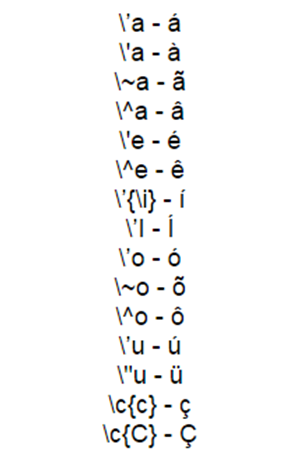
\includegraphics[scale=1.0]{USPSC-img/USPSC-AcentuacaoLaTeX.png} \\
	Fonte: \citeonline{comandos}
	\end{center}	
\end{figure}

\end{anexosenv}


%---------------------------------------------------------------------
% INDICE REMISSIVO
%--------------------------------------------------------------------
%% USPSC-IndicexRemissivosTutorial.tex
% ---
% Inicia os Índices Remissivos
% ---
%---------------------------------------------------------------------
% INDICE REMISSIVO
%--------------------------------------------------------------------
\phantompart
\printindex
%---------------------------------------------------------------------


%---------------------------------------------------------------------

\end{document}
